%TODO kohrenz->resolution? wird nicht verwendet in auswertung


\documentclass[a4paper]{scrartcl}

\usepackage[utf8]{inputenc}
\usepackage[english]{babel}
\usepackage{lmodern} 
\usepackage[T1]{fontenc}
\usepackage{booktabs}
\usepackage{multirow}
\usepackage{wrapfig}


% PAKETE
\usepackage{siunitx}
\usepackage{graphicx}
\usepackage{placeins}
\usepackage{longtable}
\usepackage{enumitem}
\usepackage{bbm}
%\usepackage{sidecap}


\usepackage{amssymb} % math symbols
\usepackage{amsmath} % ams
\usepackage{amsfonts} % mathmatical fonts

% caption indenting
 \usepackage[format=plain,indention=0em,labelfont=bf,margin=1em]{caption} 
 \usepackage{subfig} %subfigures ^^
\usepackage[protrusion=true,expansion=true]{microtype} % denser font, "-" behind line
\usepackage{esint} % nicer double and triple integrals
\usepackage{fancyhdr} % fancy headers
\usepackage[colorlinks=true,linkcolor=black,citecolor=black,filecolor=black,urlcolor=black]{hyperref}



% EINSTELLUNGEN
\sisetup{seperr,repeatunits=false}
\numberwithin{equation}{section}
\numberwithin{figure}{section}
\numberwithin{table}{section}

% EIGENE FUNKTIONEN
\newcommand{\re}{\operatorname{Re}}
\newcommand{\im}{\operatorname{Im}}
\newcommand{\gquote}[1]{\glqq #1 \grqq}

\newcommand{\eq}[2]{\begin{equation}#1\label{#2}\end{equation}}
\newcommand{\eqand}[0]{\hspace{.25cm} \bigwedge \hspace{.25cm}}
\newcommand{\grafik}[2]{\begin{figure}[h]\centering \includegraphics[width=10cm]{#1.eps}  \caption{#2} \label{#1} \end{figure} }
\newcommand{\grafikq}[3]{\begin{figure}[h]\centering \includegraphics[width=10cm]{#1.eps}  \caption[#2]{#3} \label{#1} \end{figure} }
\newcommand{\tbl}[3]{\begin{table}[h]\caption{#1}\label{#2}\begin{center}#3\end{center}\end{table}}
\newcommand{\Abbildung}[1]{\textsl{Abbildung \ref{#1}}}
\newcommand{\AbbildungI}[1]{\textsl{(Abbildung \ref{#1})}}
\newcommand{\Tabelle}[1]{\textsl{Tabelle \ref{#1}}}
\newcommand{\TabelleI}[1]{\textsl{(Tabelle \ref{#1})}}
\newcommand{\Formel}[1]{(\ref{#1})}
\renewcommand{\d}{\mathrm{d}}
\newcommand{\ve}[1]{\mathbf{ #1} }

\title{Ma 6: Atomic Force Microscopy (AFM)}
\subtitle{Tutor: Ch. Lotze}
\author{Benjamin Huber, Carolin Wille}
\date{January 2, 2012}

\begin{document}
\thispagestyle{empty}
\maketitle
\tableofcontents
\clearpage


\section{Introduction}
Atomic Force Microscopy (AFM) is a surface imaging technique, which has a very high resolution on the order of nanometers. It was developed in 1986 by Binnig, Quate and Gerber subsequently of the invention of the scanning tunneling microscope (STM) in 1981. STM, which uses the quantum mechanical tunneling current between the tip of the microscope and the sample to investigate the topography of a surface, requires conducting samples. In contrast, the AFM technique is based on very general forces, like the van-der-Waals force or chemical forces and thus allows studies of conducting as well as of non-conducting materials.

The AFM measures the forces along the sample's surface with a cantilever, on which a sharp tip is mounted. The forces influence the cantilever by either bending it towards or away from the surface. The tilting or even shearing of the cantilever is detected by a laser beam, which is reflected from the cantilever's backside towards a photo-diode. The AFM is equipped with an electronic feed-back regulation circuit, such that the distance between the tip and the sample can be held constant, which is used in some operation modus. The AFM is mounted on a piezo-element, with which the movement within the sample plane and the height can be controlled. Usually the tip moves forward line-wise like a common printer, but it always scans the lines moving in the same direction.

\begin{figure} 
 \centering
\subfloat[][Schematic Picture of an AFM]
{         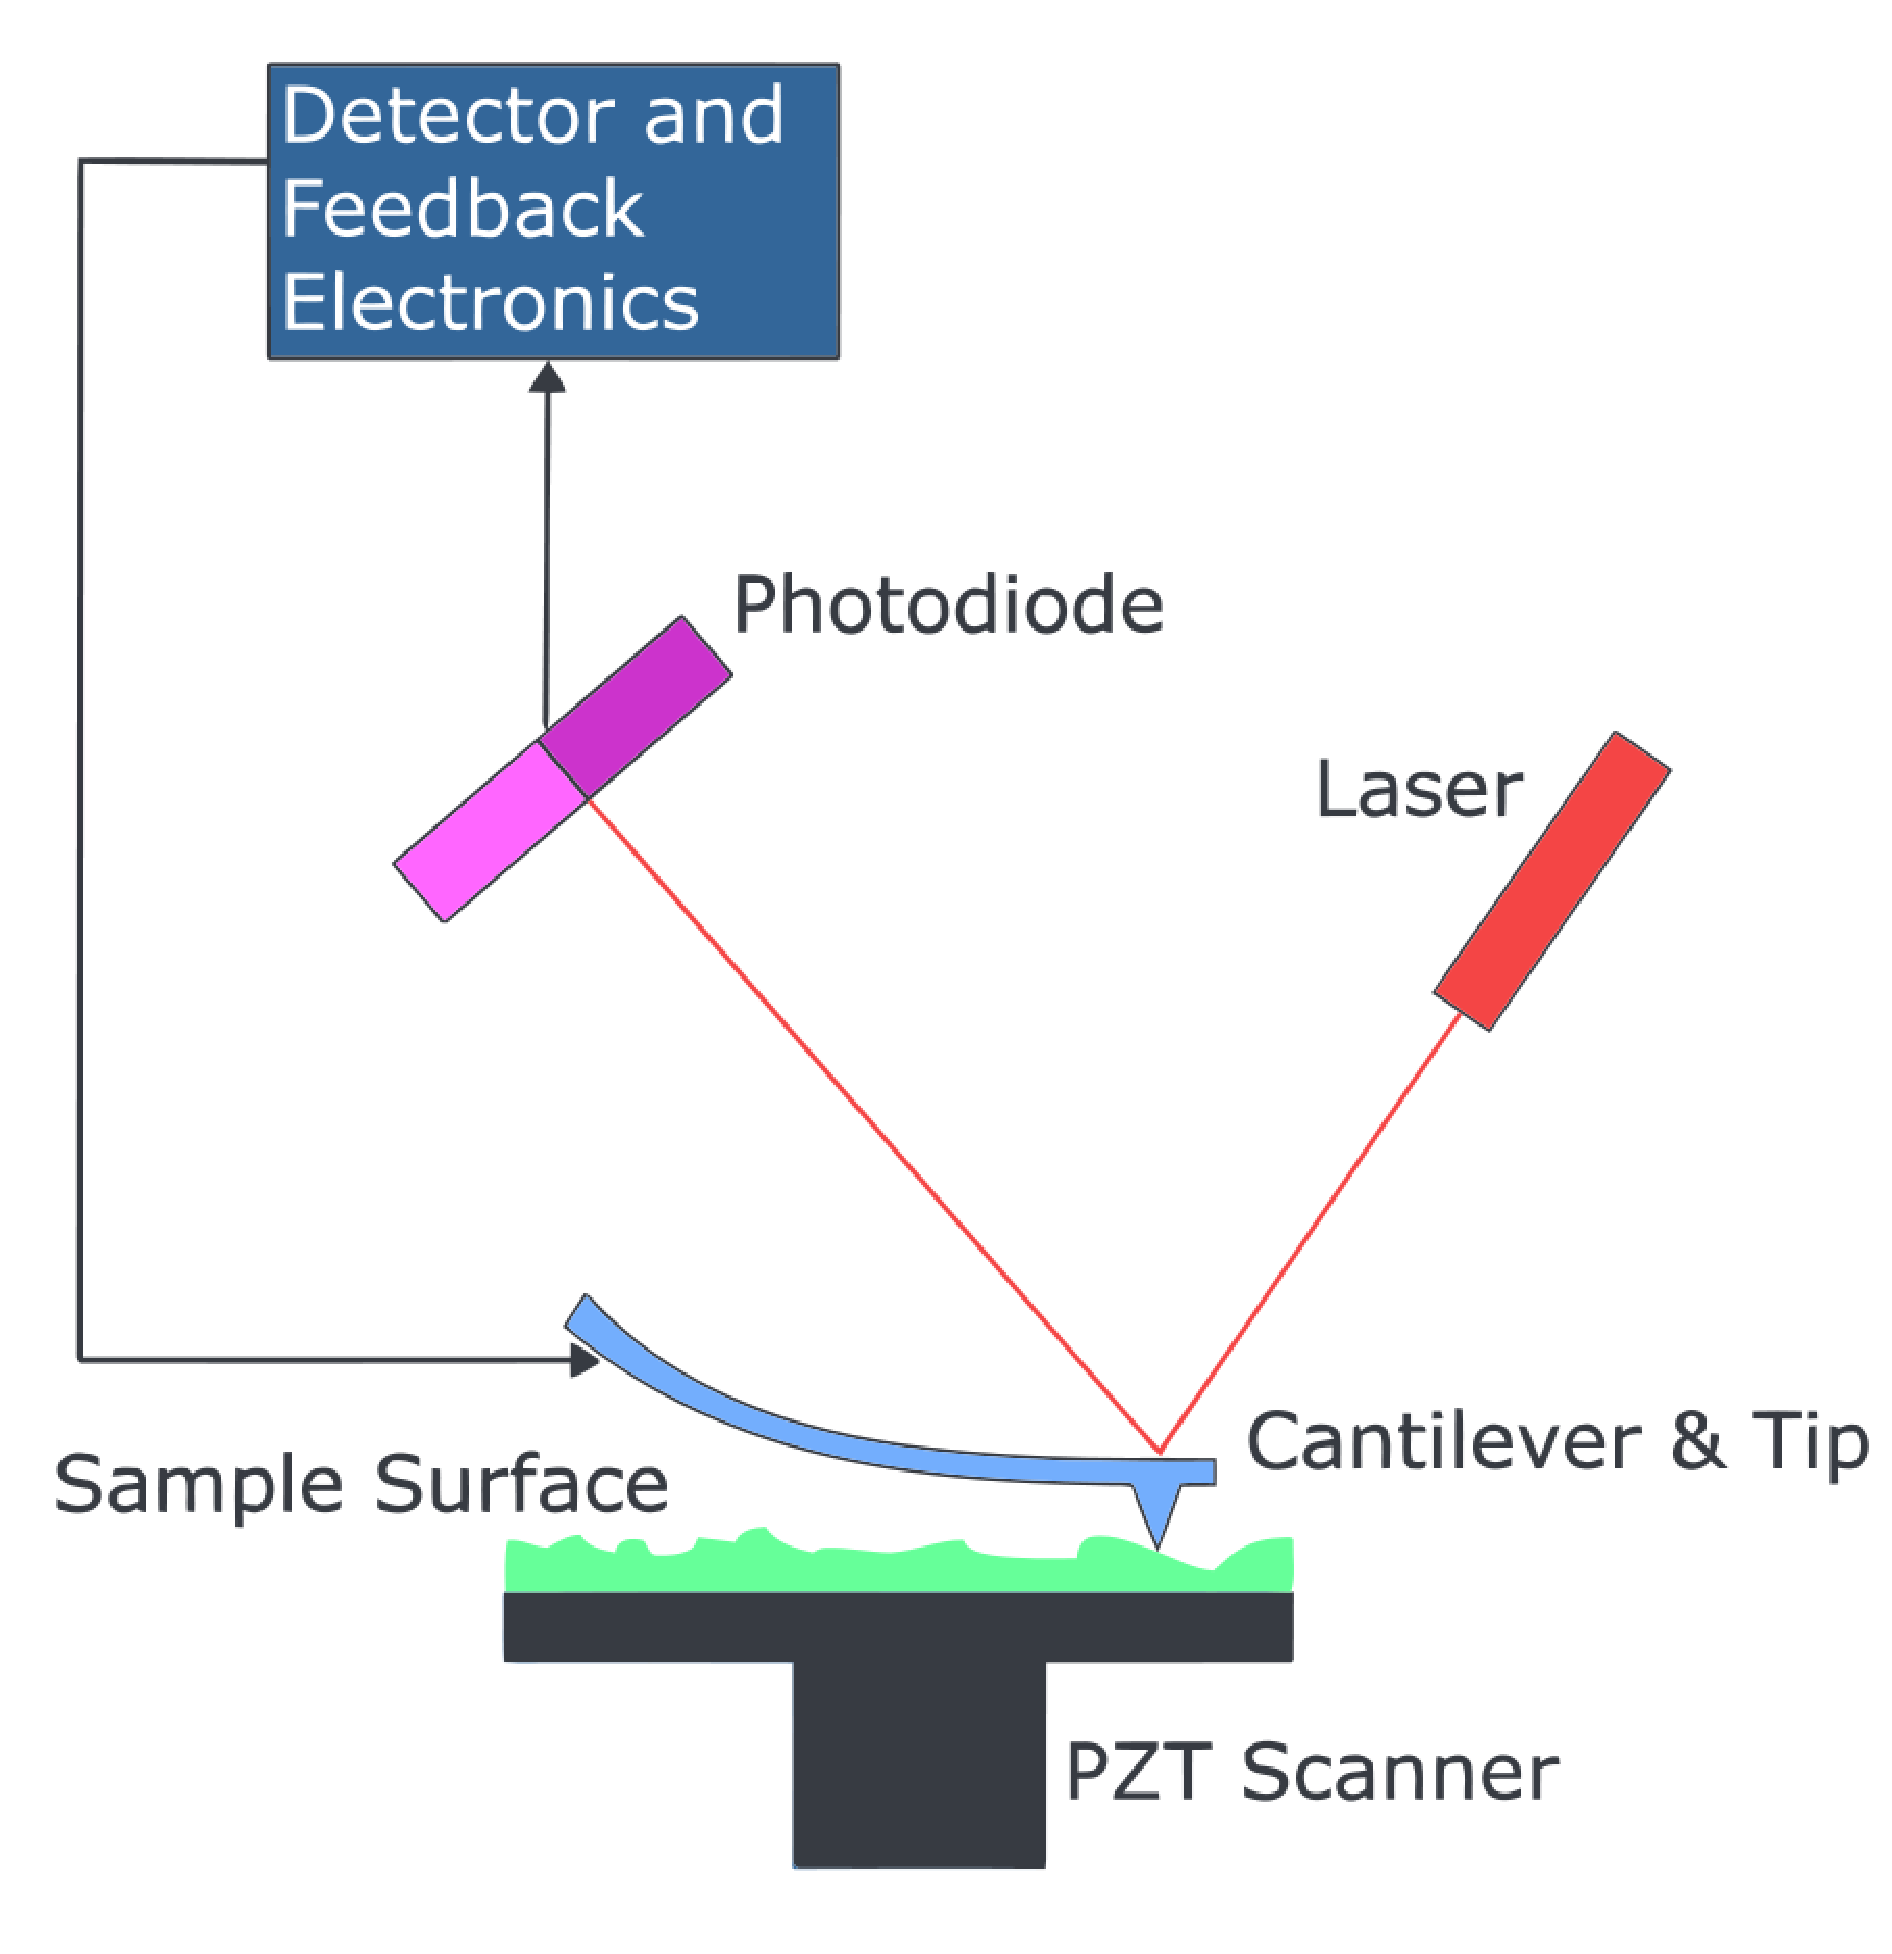
\includegraphics[width=0.4\linewidth]{img/afmsetup.pdf}
       
}
% \hfill
\subfloat[][]
       %  {\includegraphics[width=0.6\linewidth]{img/moke.pdf}}

\caption{
\small  \textbf{(a)} Typical AFM Set-Up \textbf{(b)} Source: \url{http://en.wikipedia.org/wiki/Atomic-Force-Microscope}. } 
	\label{fig:setup}
\end{figure}



\subsection{Relevant Forces acting on the AFM}
The forces acting on the AFM tip can be divided into chemical, electric, magnetic and van der Waals force
\eq{F_\text{tot}=F_\text{ch}+F_\text{el}+F_\text{mag}+F_\text{vdW} \; .} {forces}
The chemical force and the van der Waals force $F_\text{ch}$ and $F_\text{vdW}$ can be modelled by the empirical Lennard-Jones potential
\eq{V_\text{LJ}=4\epsilon\left[\left(\frac{\sigma_{0}}{r}\right)^{12}-\left(\frac{\sigma_{0}}{r}\right)^{6}\right] \; , }{jones}
where the first term describes a strong, but short ranged repulsion due to the Paul-principle acting on the overlapping electron clouds of the smaple and the tip, while the second term describes the attraction through the van der Waals force, the attraction between non-permanent dipoles in atoms. The van der Waals force acting on the tip, can be approximated by the force of a plane surface on a sphere of radius $R$ at a distance $d$ 
\begin{equation}
F_\text{vdW}=\frac{HR}{6d^{2}} \; ,
\end{equation}
$H$ is the Hamaker constant, depending on the tip-sample-combination via the atom density of both. 

The electric or Coulomb force $F_\text{el}$ can be understood in terms of a capacitor, that is formed by the tip and the sample. The voltage between the two poles is given by the contact potential
\begin{equation}
U_{contact}=\frac{1}{e}\left(\Phi_{tip}-\Phi_{sample}\right),
\end{equation}
where the $\Phi_i$ are the work functions of the respective materials. If an additional bias voltage is applied the total voltage is $U=U_\text{bias}+U_\text{contact}$ and the electric force is given by the spatial derivative of the potential 
\begin{equation}
F_\text{el}=\frac{\partial }{\partial z} \tfrac 1 2 C U^2 = \frac{1}{2} \frac{\partial C}{\partial z} (U_\text{bias}+U_\text{contact})^2 \; , \label{eq:elec}
\end{equation}
where $C$ is the capacity.

The magnetic force $F_{mag}$ is only relevant for magnetized tips and magnetic samples and is therefore not discussed here. 

\subsection{Operation Modes}  
With the typical set-up and acting forces described in the previous section, it is possible to select different operation modi of the AFM. The simplest one is the \textbf{contact mode}, where the distance between tip and sample is so small, that the repulsive Pauli force dominates. Contact mode can be used in two ways, either the height of the AFM tip is kept constant and the changes of the cantilever deflection is recorded yielding a force-profile of the surface, or the force is kept constant via regulating the height of the tip using the feed-back electronics. Thus, a height profile can be generated. However, as the distance between tip ans sample is very small in both cases, the risk of damaging both tip and sample is a big disadvantage of this modus. 

This problem can be avoided in \textbf{non-contact} mode, where the tip-sample distance is in the attractive force regime. To avoid spontaneous crashes into the sample in regions with high attractive forces, the cantilever is made of sufficiently hard materials. In non-contact mode the cantilever is not gliding statically over the sample surface, but is driven to oscillate at a frequency close to its own resonance, therefore non-contact mode is also referred to as dynamic mode.

\begin{figure} 
 \centering
\subfloat[][Force between tip and sample]
         {\includegraphics[width=0.6\linewidth]{img/forces.png}}
\caption{
\small \textbf{(a)} Force acting on the AFM tip vs tip-sample distance. Different distances and the corresponding signs of the force (repulsive/attractive) are used in the two different operation modi (contact/non-contact).
Source: \url{http://en.wikipedia.org/wiki/Magneto-optic_Kerr_effect}. } 
	\label{fig:forces}
\end{figure}



The equation of motion of the tip-sample distance can be modeled as a damped, driven harmonic oscillator with an additional attractive force $F_a$
\begin{equation}
m\ddot{z}+\gamma \dot{z}+kz=F_{0} \exp( {i \Omega t})+F_{a} \label{eq:differential}
\end{equation}
where $z$ is the oscillation amplitude around equilibrium position, $m$ is the mass, $\gamma$ is the damping factor, $k$ is the spring constant , $F_0$  the amplitude and $\Omega$ the frequency of the driving force. The oscillation frequency is given by $\omega_0\,=\,\sqrt{k/m}$. If the oscillation amplitude is small, it is reasonable to expand the attractive force in powers of the oscillation amplitude. The constant term leads to a shift of the equilibrium position and is not important. The linear term can be included into an effective spring constant
\begin{equation}
k_\text{eff}=k-\frac{\partial F_{a}}{\partial z} \label{eq:change}.
\end{equation}
This shift corresponds to a shift of the resonance frequency and therefore can be connected to a change of the oscillation amplitude. From equation \Formel{eq:differential} the oscillation amplitude can be derived to be
\begin{equation}
A=\frac{A_{0}}{i\gamma\Omega+\omega_{0}^{2}-\Omega^{2}},
\end{equation}
where $A_0=F_0/m$ is the amplitude of the oscillator without the driving force. This amplitude is a complex number. The phase can be interpreted as a phase shift, the magnitude is the amplitude we wanted:
\begin{equation}
|A|^{2}=\frac{a_{0}}{(\omega_{0}^{2}-\Omega^{2})^{2}+\gamma^{2}\Omega^{2}}=\frac{a_{0}}{(\omega_{0}^{2}-\Omega^{2})^{2}-\gamma(\omega_{0}^{2}-\Omega^{2})+\gamma^{2}\omega_{0}^{2}}.
\end{equation}

Introducing the quality factor of the cantilever $Q=\omega_0/2\gamma$ and the relative amplitude $a=A_0/A$ we can now calculate the Force gradient
\begin{equation}
\frac{\partial F_{a}}{\partial z}=k\left(\frac{1-2a^{2}+\sqrt{4Q^{2}\left(a^{2}-1\right)+1}}{2\left(Q^{2}-a^{2}\right)}\right)
\end{equation}







\clearpage
 \bibliographystyle{unsrt}
\bibliography{bib}

\end{document}


